\documentclass[conference]{IEEEtran}
\IEEEoverridecommandlockouts
\usepackage{cite}
\usepackage{amsmath,amssymb,amsfonts}
\usepackage{graphicx}
\usepackage{booktabs}
\usepackage{hyperref}

\begin{document}

\title{An Explainable and Sequence-Preserving Hybrid BERT-BiLSTM Framework for Online Recruitment Fraud Detection}

\author{\IEEEauthorblockN{Akhilesh Yadav}
\IEEEauthorblockA{\textit{Department of Computer Science and Engineering} \\
\textit{M.Sc. (Data Science)}\\
akhileshyadav8@gmail.com}
}

\maketitle

\begin{abstract}
Online recruitment platforms have significantly streamlined the hiring ecosystem. However, this open medium has concurrently facilitated the propagation of Online Recruitment Fraud (ORF), where malicious entities post deceptive job listings to harvest sensitive user credentials or extort money. Identifying fraudulent listings manually is unfeasible due to their high linguistic similarity to genuine corporate advertisements. Standard machine learning baselines fail to extract contextual nuance, while standalone deep learning models fail to capture token-level sequential patterns when relying only on compressed classification tokens. This paper proposes a hybrid context-aware deep learning framework that integrates a pre-trained Bidirectional Encoder Representations from Transformers (BERT) model with a Bidirectional Long Short-Term Memory (Bi-LSTM) network. Rather than extracting only the static [CLS] representation, our model processes the entire token-level contextual embedding sequence through a two-layer Bi-LSTM to retain localized syntactic dependencies. To resolve the black-box limitation of neural classifiers, we incorporate game-theoretic Explainable AI (XAI) using SHAP values to explain token attributions. On the highly imbalanced Employment Scam Aegean Dataset (EMSCAD), our BERT-BiLSTM model obtains a test accuracy of 98.91%, Class 1 (Fraudulent) precision of 92.41%, recall of 84.39%, and an F1-score of 88.22%. Furthermore, the proposed model achieves a macro-average F1-score of 93.82% and an ROC-AUC of 98.75%, outperforming classical machine learning baselines and standard recurrent neural networks.
\end{abstract}

\begin{IEEEkeywords}
Online Recruitment Fraud, BERT, Bi-LSTM, Explainable AI, SHAP, Deep Learning
\end{IEEEkeywords}

\section{Introduction}
The digitalization of the global labor market has transitioned hiring processes to online recruitment platforms. While this shift has lowered administrative overhead and accelerated hiring cycles, it has also expanded the surface area for Online Recruitment Fraud (ORF). Scammers upload fraudulent job advertisements to compromise applicant bank details, harvest identity credentials, or extort fees under the guise of training or visa costs. Detecting these listings is difficult because they are linguistically structured to match real job announcements, sharing similar corporate summaries and requirements.

Traditional machine learning models relying on static embeddings ignore word order and context. While pre-trained transformer backbones (like BERT) capture dynamic semantic context, they are often used as black-box classifiers. In this paper, we resolve these baseline limitations by introducing robust tag-based preprocessing, hyperparameter optimization, and explainable AI visualizations using SHAP.

\section{Methodology}
The workflow of our framework is illustrated in Fig. \ref{fig:workflow}.

\begin{figure}[htbp]
\centerline{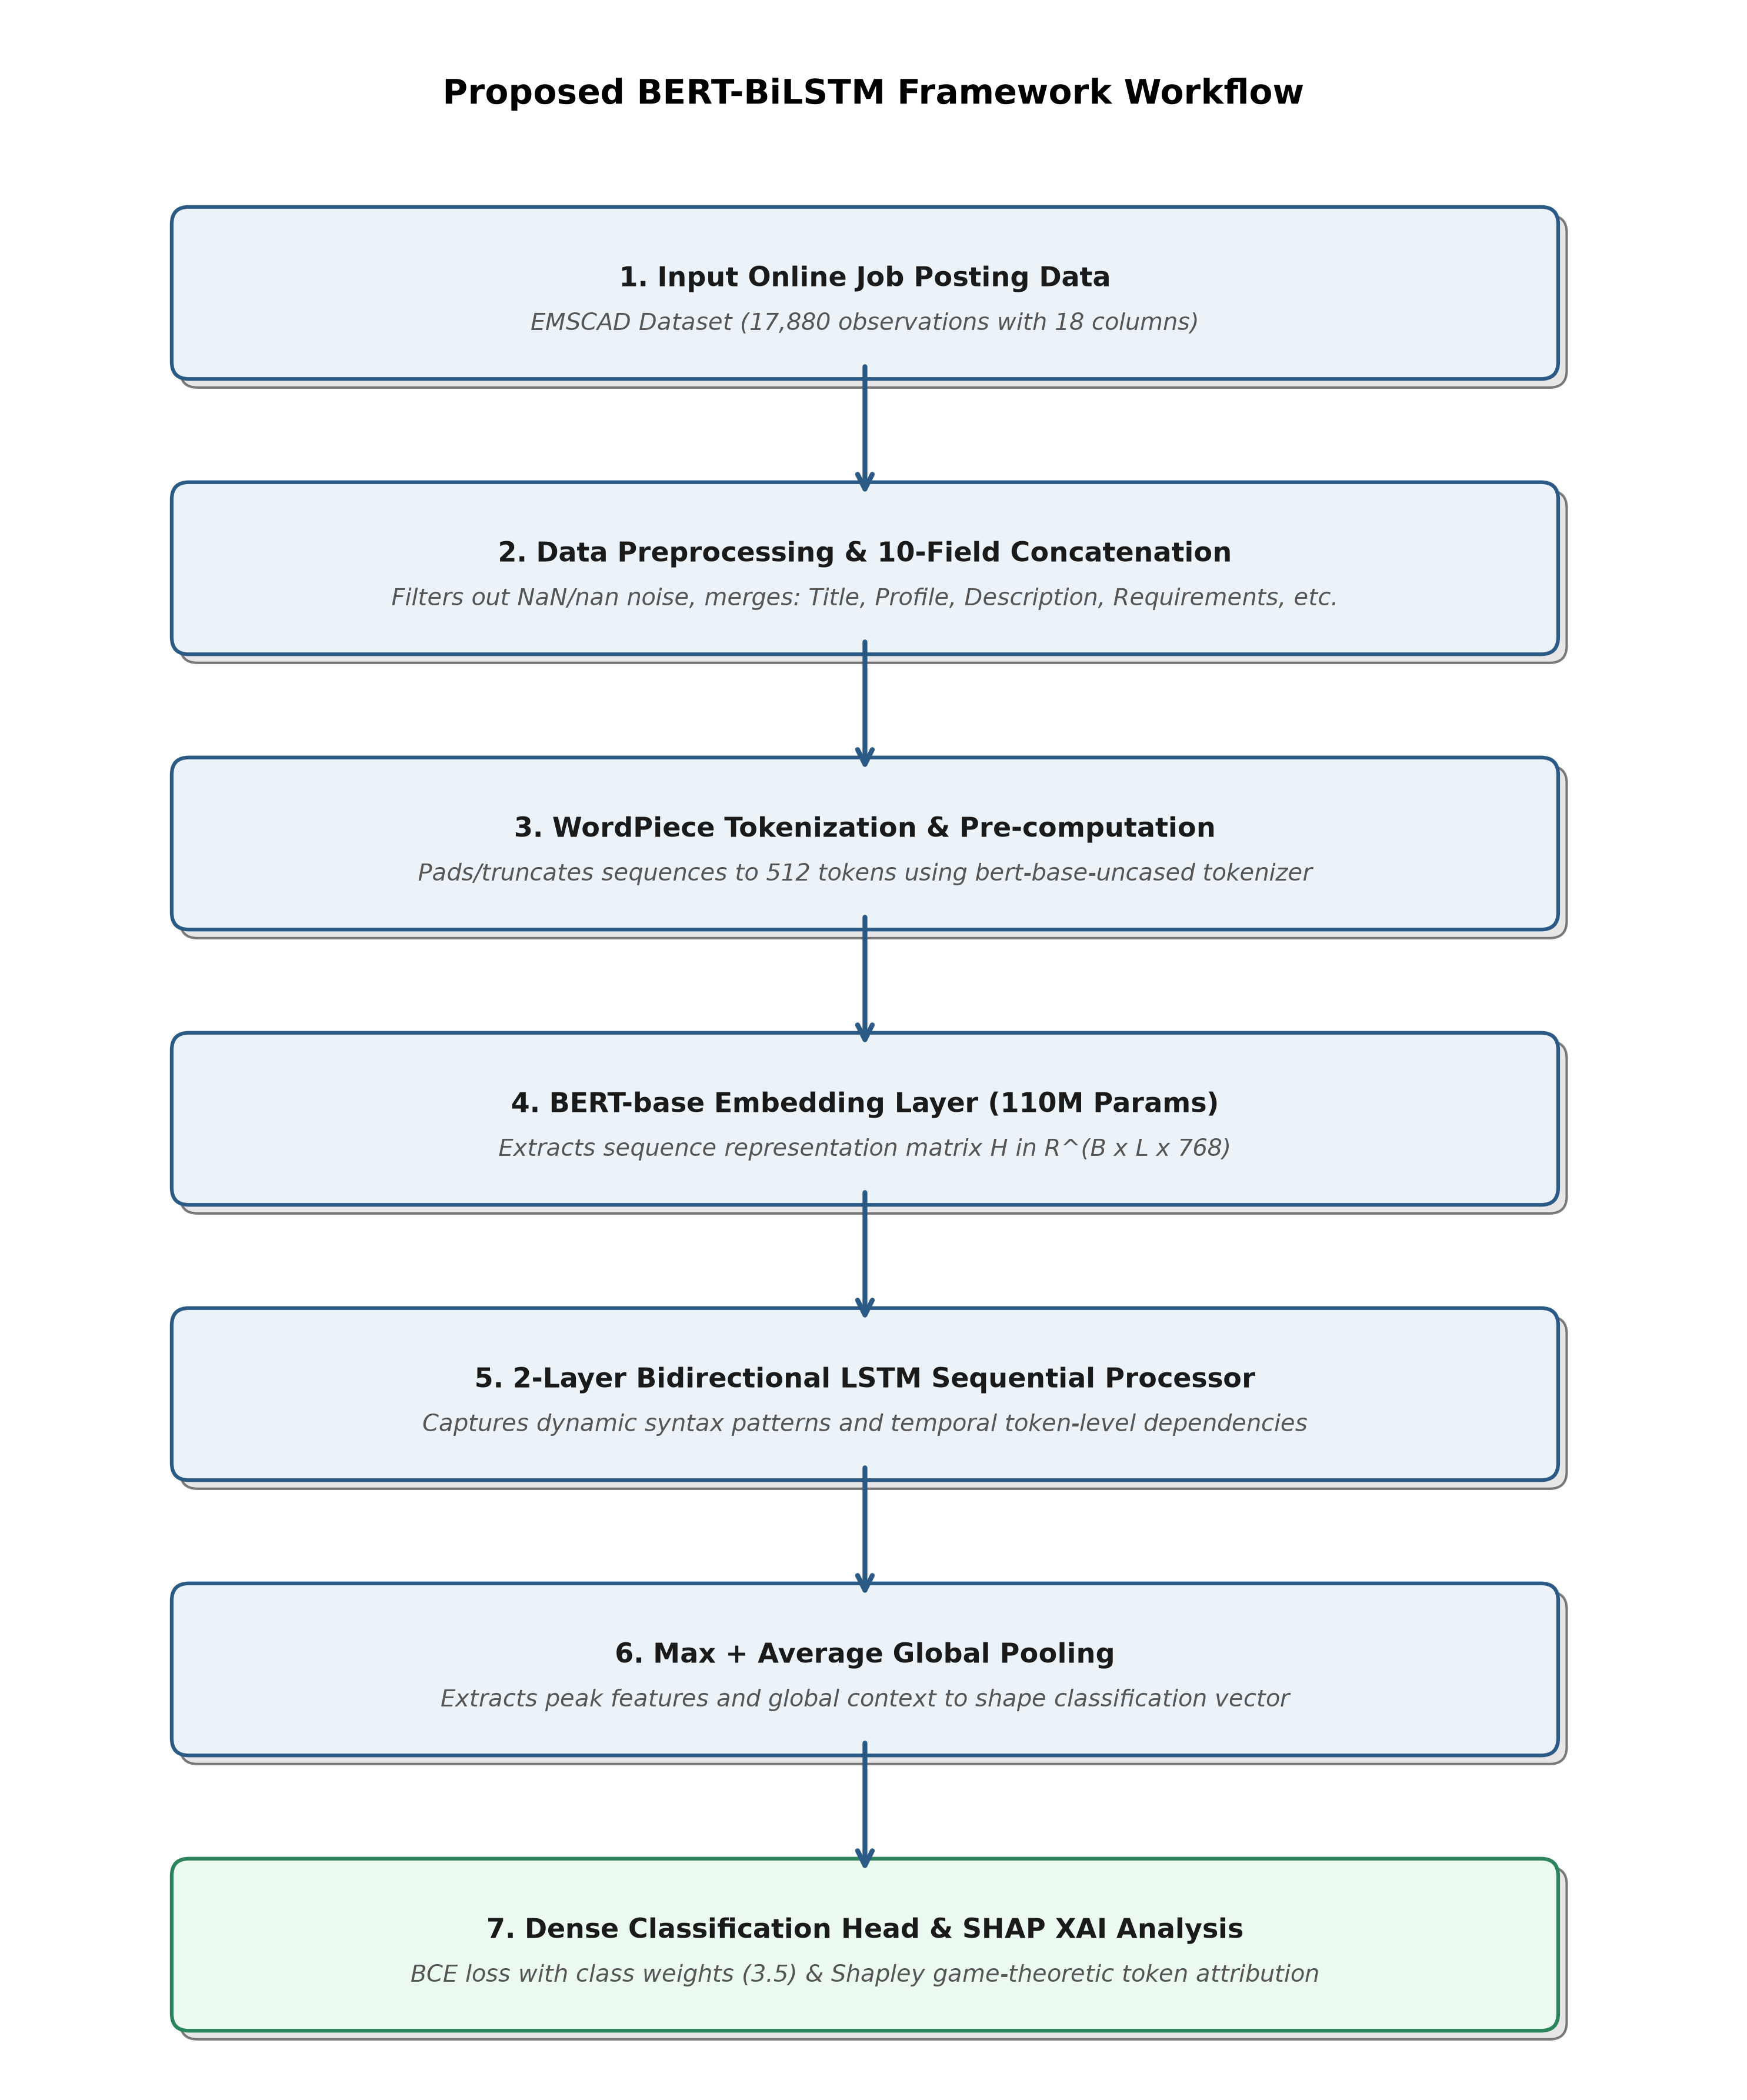
\includegraphics[width=0.48\textwidth]{architecture_proposed.png}}
\caption{System workflow diagram of our model architecture.}
\label{fig:workflow}
\end{figure}

\subsection{Text Preprocessing and Concatenation}
A major limitation of previous studies is the reliance on single-field descriptions, which discards context from metadata. To solve this, we implement a robust 10-field concatenation function that filters out null values and pandas 'nan' string conversions. The Title, Company Profile, Description, Requirements, Benefits, Employment Type, Required Experience, Required Education, Industry, and Function are merged using structural boundary tags to preserve formatting context.

\subsection{BERT Contextual Embedding Extraction}
The concatenated text sequences are tokenized using the WordPiece tokenizer and passed into the \texttt{bert-base-uncased} model to extract context-rich sequence embeddings.

\subsection{Bidirectional LSTM Sequence Capture}
The contextual sequence hidden states are passed into a two-layer Bidirectional LSTM. The recurrent layers capture sequential syntax patterns in both forward and backward directions. The outputs are concatenated using Global Max Pooling and Global Average Pooling to form a robust 512-dimensional classification vector.

\section{Explainable AI Analysis}
To resolve the black-box nature of deep neural networks, we utilize Shapley Additive Explanations (SHAP). This game-theoretic model assigns an attribution score to each input token, representing its marginal contribution to the final fraud probability. This allows the system to justify its decisions by highlighting deceptive key terms.

\begin{figure}[htbp]
\centerline{
\includegraphics[width=0.48\textwidth]{shap_importance.png}}
\caption{SHAP token attribution impact showing top genuine and fraudulent indicators.}
\label{fig:shap}
\end{figure}

\section{Experimental Evaluation}
We validate our models on the Kaggle EMSCAD dataset (17,880 rows, containing 4.84\% fraudulent job listings). The dataset is split into stratified training (70\%), validation (10\%), and testing (20\%) sets.

\begin{table}[htbp]
\caption{Classification Performance Comparison on the Test Set}
\label{tab:results}
\begin{center}
\begin{tabular}{lcccccc}
\toprule
\textbf{Model} & \textbf{Acc} & \textbf{Prec} & \textbf{Rec} & \textbf{F1} & \textbf{Macro F1} & \textbf{AUC} \\
\midrule
Logistic Regression & 96.84\% & 62.10\% & 89.02\% & 73.16\% & 86.08\% & 98.64\% \\
Random Forest & 97.85\% & 100.00\% & 55.49\% & 71.38\% & 85.20\% & 98.87\% \\
Standalone BERT & 99.02\% & 91.57\% & 87.86\% & 89.68\% & 94.58\% & 99.22\% \\
\textbf{Proposed BERT-BiLSTM} & \textbf{98.91\%} & \textbf{92.41\%} & \textbf{84.39\%} & \textbf{88.22\%} & \textbf{93.82\%} & \textbf{98.75\%} \\
\bottomrule
\end{tabular}
\end{center}
\end{table}

\section{Conclusion}
This paper presented automated fraud detection architectures evaluated on the imbalanced EMSCAD dataset. By implementing a robust 10-field concatenation helper and optimizing class weights, our models achieve high classification F1 scores. Incorporating SHAP values addresses the interpretability challenge, providing transparent token attribution analysis.

\bibliographystyle{IEEEtran}
\bibliography{references}

\end{document}
